\section{Multiobjective Development Evaluation}
\subsection{Problem and mechanism}
The next independent development batches retain strict CPD improvement as one mode, but do not require every retained final candidate to beat strong A0 in CPD. Two complementary questions are posed: can timing improve within registered resource limits, and can routed wirelength or actual vertical occupancy decrease within a registered timing range? Fixed CPD, wirelength, SB-pair and CB-source limits are design parameters anchored at the original batch state. They are not rolling tolerances or research termination conditions. The current already-registered observations and their historical acceptance rules remain unchanged.

The proposed combined intervention uses measured capacity competition to select noncritical owners of scarce resources, uses their timing margin to reconnect them elsewhere in a transaction copy, and then repairs critical or near-critical connections. Occupancy is updated after every step; native FULL, physical resource accounting and complete STA govern the final commit or rollback. A temporary release need not independently improve CPD. Final non-dominated retention is distinct from intermediate search transitions. At present the fixed-budget policy arithmetic and historical-state replay are implemented; the new capacity-release mechanism has not yet produced a new native result.

\subsection{Overall states and joint Pareto tradeoffs}
The initial archive contains 85 actual run or observation records: 45 formal-timing repetitions, 12 strong A0/R1/Tf reconvergence runs and 28 exact-vector initial or repair states. They include duplicates of the same physical route and unequal convergence/repair opportunities, so they are not 85 independent quality samples. Every record keeps its actual input hashes, binary, command, convergence setting, route, physical audit and time scope. The descriptive four-dimensional archive minimizes CPD, planar routed wirelength, used SB pairs and used CB output sources. It retains 43 records with no observed dominator and 10 additional records whose dominance is unresolved by six-significant-digit CPD reports; 32 are dominated in these four dimensions. Dominated records remain in the evidence. Missing standalone repair time is never replaced by zero or by an analysis-only process time.

\begin{figure*}[t]
\centering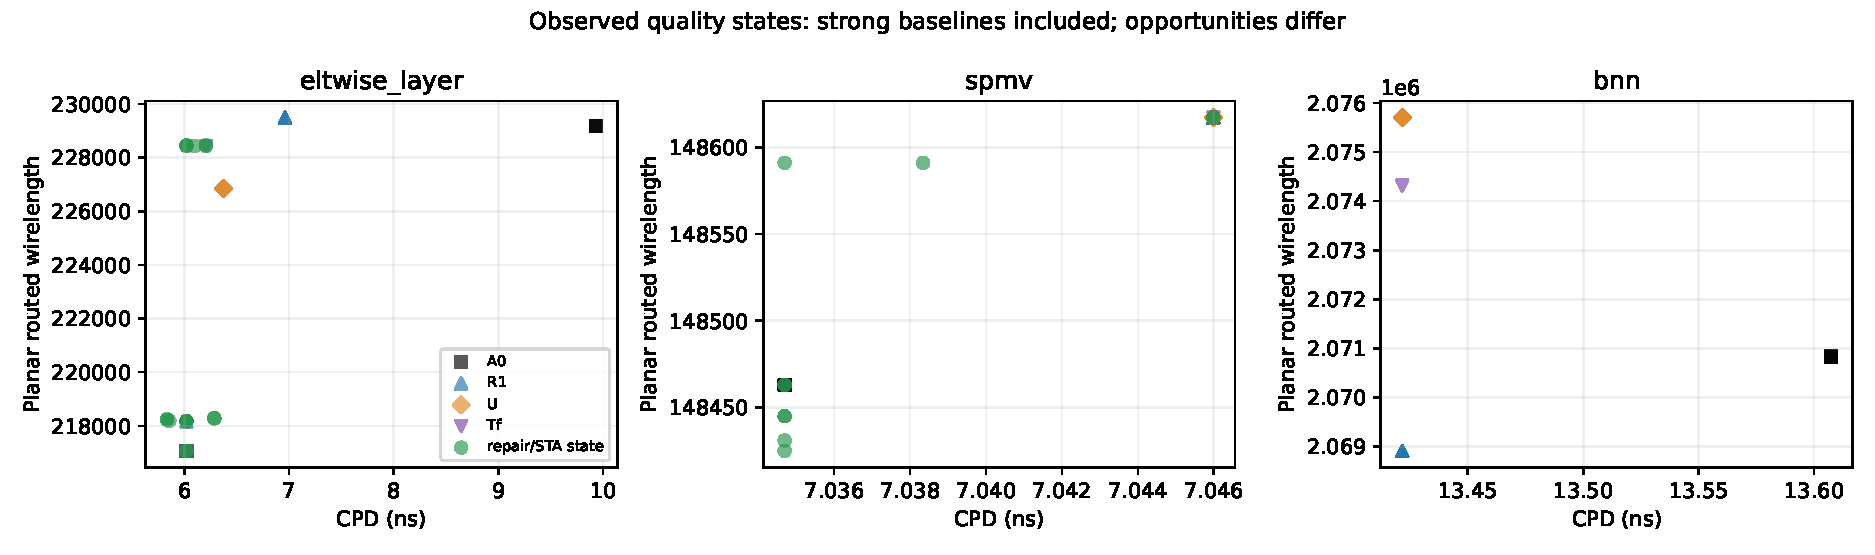
\includegraphics[width=\textwidth]{data/multiobjective_quality_projection_v14.pdf}
\caption{Observed joint-population quality projections, including strong baselines. These project CPD/wire from a four-dimensional resource archive; they neither establish two-dimensional dominance nor equal-opportunity algorithm superiority. Repeated states may overlap.}
\label{fig:multiobjective-development}
\end{figure*}

Several previous outcomes change interpretation. The legal SPMV weighted joint candidate rejected by both timing policies has CPD 7.034697713237392 ns, wirelength 148431, one SB pair and 967 CB sources. Its endpoint vector was unchanged, but its wirelength is 32 below strong A0 at the expense of one additional SB pair. It also uses 14 less wirelength than the accepted endpoint-improving plateau at equal CPD/SB/CB, and therefore dominates that plateau in this four-dimensional projection. The plateau's improved endpoint vector remains a separate benefit not represented by the four archive dimensions. A different strict-rejected physical joint candidate has the same CPD, wirelength 148425 and three SB pairs. Both remain eligible resource tradeoffs; neither small wirelength gain is described as a large engineering improvement. SPMV initial R1, U and Tf states at 7.04599 ns, wirelength 148617 and one SB pair are quality-dominated by strong A0.

For eltwise, strong A0 has approximately 6.018101 ns CPD, wirelength 217065, 30 SB pairs and 968 CB sources. The automatic R1 repair state reaches 5.832275 ns with wirelength 218245, 40 SB pairs and 970 CB sources: a timing/resource tradeoff, not an all-resource win. The Tf initial state at approximately 6.20812 ns, wirelength 228420, 118 SB pairs and 955 CB sources survives because its CB-source occupancy is lower. Such mathematical non-dominance alone does not establish an attractive engineering choice. The earlier U state is quality-dominated by strong A0, but its different convergence conditions prevent transferring that conclusion to complete runtime.

BNN provides a more promising cost/resource comparison. In the matched formal-timing cohort, R1 and U have the same reported 13.4216 ns CPD. U has wirelength 2075701, 94 SB pairs and 5066 CB sources, versus R1's 2068908, 86 and 5072. Their three-repeat complete-process medians are respectively 283.605 and 549.419 s. This is an observed whole-process tradeoff within that older formal cohort, not a current repair-prototype timing claim. Strong native reconvergence A0, R1 and Tf are separate points; Tf has wirelength 2074317, 105 SB pairs and 5062 CB sources at the same reported CPD as R1, with distinct resource tradeoffs. Their new high-precision initial observations are retained separately.

\subsection{Mechanism-specific controls and selection}
Subsequent native controls receive the same current-STA selector, full-device search domain, modifiable tree scope and repair opportunities. Release-only, repair-only and combined interventions distinguish scarce-resource release from extra search or scheduling. Combinations are allowed when their mechanisms depend on each other; ablations test the corresponding claim rather than requiring every component alone to improve CPD. Confirmation freezes a version and a circuit-independent selection rule. Development Pareto points are not converted into a per-circuit historical-best configuration.

An independent arithmetic replay evaluates 6720 fixed-budget conditions on existing exact-vector states, with seven distinct states meeting at least one condition. This is policy eligibility, not 6720 routing experiments, seven new improvements or newly committed states. CPD limits are checked at full precision with no epsilon; a value one representable step above the fixed limit is rejected. The resource objective can be wirelength, SB or CB, with the other dimensions held to their registered limits. The separate archive may retain tradeoffs rejected by a particular transition policy.

\subsection{Complete cost and limitations}
Twenty native transaction core-time receipts are linked to their existing candidate records. Core time is nested within the repair wrapper; subsequent candidate FULL/STA and the shared strict/endpoint research workflow are separate scopes. A complete standalone single-configuration repair-algorithm time, including failed candidates and rollback, is still unknown for these archived states. The 45 U-era formal measurements remain attached only to their original runs. Actual-graph cache construction, current-state construction, query failures and validation costs will be included in new end-to-end measurements.

This organization follows the joint QoR, hyperparameter tradeoff, ablation and runtime evaluation in Escaping Flatland~\cite{flatland}, while retaining our fixed-placement routing boundary. Occupancy reduction on a fixed architecture is not a demonstrated chip-area or power reduction. BNN graph preparation and slack-release screening are now registered independently; the three pristine A0/R1/Tf timing-cone observations have completed without routing changes. No research-wide date, invocation limit or terminating matrix is introduced.
